\chapter{Grundlagen} \label{chapter_2}

In diesem Kapitel werden die gezielten Anforderungen der Arbeit geschildert, die Anwendungsdomäne erläutert und der Konfigurator Merlin Enterprise vorgestellt. 

\section{Produktkonfiguratoren} 
Das Ziel des Produktkonfigurators ist es, produktspezifisches Wissen für die Anwender bereit zu stellen, die ihn dabei unterstützt sein Produkt individuell zusammenzustellen. Ein solches System wird in die Kategorie der Expertensysteme\cite{bib:puppe} oder wissensbasierte Systeme eingeordnet . Der Aufbau eines solches System ist in Abbildung \ref{expert_system_structure} zu sehen. \par
\begin{figure}[hb]
\centering
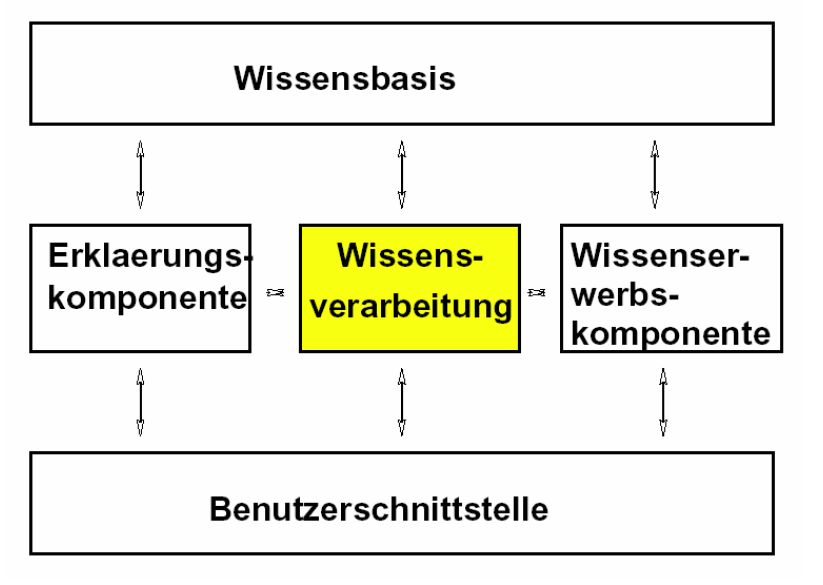
\includegraphics[width=250px]{images/expertensysteme}
\caption{Aufbau eines Expertensystems \cite[s.6]{bib:keller}}
\label{expert_system_structure}
\end{figure}


\section{CAS Configurator Merlin Enterprise} \label{configurator}
Das Produkt CAS Configurator Merlin Enterprise ist die Konfigurationslösung der CAS Software AG für große Unternehmen. Das Produkt selbst ist kein Standardprodukt, da die einzelnen Komponenten für jeden Kunden an die jeweiligen Bedürfnisse angepasst werden. Der Konfigurator ist ein Expertensystem, welches, nach 


\section{Umfeld der Arbeit}
Die Arbeit wird in der Anwendungsdomäne Luftfahrt durchgeführt. Für den derzeitigen Produktkonfigurator, der in Abschnitt \ref{configurator} genauer beschrieben wird, besteht bereits ein Webinterface. Das komplette Produkt ist beim Kunden Airbus im Einsatz.  


\section{Grundlegende Anforderungen}
Die Anwendung ist kein konkretes Kundenprojekt. Dies hat zur Folge, dass es keine strikten Anforderungen für die App gibt. Die Anwendung soll, wie in Abschnitt \ref{goal} festgelegt den Konfigurationsprozess vereinfachen und "mobil" verfügbar machen. Der Prototyp soll den Kunden überzeugen, seinen derzeitigen Konfigurationsprozess in den Neuen zu überführen. Die Anforderungen an die Software müssen demnach so festgelegt werden, dass sie für eine hohe Akzeptanz beim Kunden sorgt. Alle Gütekriterien der Anwendung müssen dieses Ziel verfolgen. \par

Die Festlegung der Kriterien ist nach Rücksprache mit den Entwicklern und dem Projektleiter des entsprechenden Kunden entstanden. Gemeinsam wurde ebenfalls eine Priorisierung der einzelnen Anforderungen erarbeitet. Im Folgenden ist das Ergebnis in Funktional und Nicht-Funktional eingeordnet. Die funktionalen Anforderungen sind die bereits vorhandenen Möglichkeiten der bestehenden Software. Diese wurden mit zusätzlichen Anforderungen, welche durch die mobile Umgebung notwendig sind ergänzt. Bei den Nicht-Funktionalen Kriterien steht die Usability, die Optimierung auf die mobile Umgebung, sowie die Kundenbegeisterung im Vordergrund.

\subsection{Nicht-Funktionale Anforderungen}
\begin{tabular}{| p{1.1cm} | p{2.2cm} | p{4.3cm} | p{4.9cm} | p{1.3cm} |}
\toprule[2pt] \rowcolor{dunkelgrau}
\hline
  Kürzel & Anforderung & Beschreibung & Details & Priorität \\
  \hline
  B1 & Einfache \newline Bedienung & Die Anwendung soll von unerfahrenen Benutzern schnell bedient werden können.& Schwerpunkte der Softwareergonomie\cite{bib:softwareErgonomie}: 
  \begin{itemize}
        \item Selbstbeschreibungs-fähigkeit
        \item Lernförderlichkeit
        \item Erwartungs-konformität
     \end{itemize}
   & A \\
  \hline
  B2 & Schnelle Bedienung & Die Auswahl der einzelnen Komponenten soll möglichst schnell getätigt werden können. & Es muss für eine flüssige Navigation zwischen den einzelnen Seiten gesorgt werden. Der Benutzer sollte keine langen Wartezeiten beim Bedienen der Anwendung haben. Ebenfalls sollten Inhalte schnell gefunden werden können. & A \\
  \hline
    B3 & Offline-Online Modus & Die Anwendung soll einen offline, sowie einen online Modus enthalten & Daten sollen Konfigurationsdaten offline zusammengestellt werden können, die später oder zeitgleich online (mit Konfigurationsserver) geprüft werden können. & A \\
    \hline
    B4 & Allein-stellungs-merkmal & Um den Kunden zu begeistern ist ein besonderes Feature, welches die Anwendung als Alleinstellungsmerkmal besitzt wünschenswert.& Es sollen besonders "'aufregende"' Features, die eine Technologie bietet in die Anwendung integriert und in einem sinnvollen Kontext genutzt werden.  & B\\
    \hline
\bottomrule[2pt]
\end{tabular}

\section{Abgrenzung der Arbeit}




